\chapter{Implementierung Device}
\label{cha:impl_device}

\section{Technologische Grundlagen}
\subsection{Android}
%TODO evtl. ein kurzer Abschnitt über Android, Java, die App auf der Brille?

\subsection{Visualisierung der Regale}
Für einige Prozesse auf der Brille ist es erforderlich, dass die exakte Position eines Produktes in einem Regal auf der Verkaufsfläche angezeigt wird. Dazu gibt es unter Verwendung von Wearable Computern grundsätzlich zwei Möglichkeiten:

\begin{enumerate}
	\item Das Regal wird abstrahiert und schematisch in einer vereinfachten Form dargestellt. Innerhalb dieser Darstellung wird die Position des gesuchten Produktes im Regal markiert. Der Benutzer muss selbst die Verknüpfung zwischen der Darstellung und der Realität herstellen, wenn er vor dem Regal steht.
	\item Durch Nutzung einer Videokamera wird die Umgebung des Benutzers und somit das Regal digital erfasst und durch Bild-im-Bild-Überlagerung die Produktposition im Regal markiert. Die Verknüpfung von Darstellung und Realität ist dadurch sehr stark. Voraussetzung ist hierbei jedoch, dass der Benutzer sich direkt vor dem Regal befindet -- andernfalls ist wiederum eine abstrahierte Darstellung erforderlich.
\end{enumerate}

Für die Umsetzung des Systems im Rahmen dieser Arbeit wurde die erste Möglichkeit gewählt, da sie technisch einfacher umzusetzen ist und zugleich auch eine Umsetzung der zweiten Möglichkeit vorbereitet.

Für die schematische Darstellung des Regals wurde die Ansicht gewählt, die ein Benutzer hat, wenn er sich vor dem Regal befindet (Frontalansicht oder Draufsicht). Regale sind rechteckig, ebenso wie Regalfächer, und lassen sich jeweils über Höhe und Breite, sowie bei den Fächern über die Position im Regal beschreiben. Dies sind optimale Voraussetzungen für die Umsetzung als zweidimensionale Ansicht.

Die technische Umsetzung der schematischen Darstellung kann i.A. auf drei Arten erfolgen:

\begin{enumerate}
	\item als Bitmap (pixelbasierte Grafik);
	\item als Vektorgrafik, also eine mathematisch beschriebene Grafik, die bei Ausgabe auf Bildschirmen verlustfrei in eine Bitmap der gewünschten Auflösung umgewandelt wird; oder
	\item als \acs{3D}-Grafik, die zusätzlich noch Tiefeninformationen speichert.
\end{enumerate}

Für die Darstellung auf dem Gerät fiel die Entscheidung auf eine Umsetzung als Vektorgrafik im \acs{SVG}-Format. Eine \acs{SVG}-Grafik ist im Grunde eine \acs{XML}-Datei, besteht also aus Text. Grundformen wie Rechtecke lassen sich über \acs{SVG} sehr einfach beschreiben, und für die Darstellung eines Regals werden keine komplizierteren Formen benötigt. Dies ist sehr platzsparend im Vergleich zu Bitmaps mit dem selben visuellen Inhalt. Außerdem können im \acs{XML}-Code der \acs{SVG}-Grafik weitere Informationen über das Regal und die Fächer hinterlegt werden, wie z.B. die entsprechenden IDs der Fächer und Produkte aus der Datenbank. Nicht zuletzt ist die verlustfreie Skalierbarkeit der Vektorgrafik ein unschätzbarer Vorteil, der das Grafikformat unabhängig von der Größe der Ausgabe macht und somit die Geräteunabhängigkeit der Applikation wesentlich verbessert.

Für SMAR sind daher alle Regale als \acs{SVG}-Grafiken angelegt. Die Grafiken werden bei Anlegen eines Regals in der Webadministration automatisiert erzeugt und in einer eigenen Tabelle (\textbf{\textit{shelf\_graphic}}) gespeichert. Bei Updates für ein entsprechendes Regal (z.B. Bearbeiten des Regals oder von darin enthaltenen Fächern) wird die \acs{SVG}-Grafik neu generiert und in der Tabelle aktualisiert. Die Grafik selbst enthält neben der Darstellung auch die IDs der Fächer, um diese später einfach ansprechen zu können.

Die Smartglass selbst lädt sich bei Start der App automatisch den neuesten Stand der \acs{SVG}-Grafiken aus der Datenbank herunter und speichert die Grafiken lokal als Dateien ab. Wird eine Regal-Darstellung benötigt, kann diese direkt aus dem lokalen Speicher der Smartglass geladen werden. Dies spart während der Nutzung der Brille Traffic und erhöht somit die Performance der Anwendung. Soll außerdem ein Regalfach markiert werden, kann direkt der \acs{XML}-Code der \acs{SVG}-Grafik manipuliert werden -- z.B. kann über die angeheftete ID eines Faches die entsprechende Rechteck-Form gesucht und über entsprechende \acs{SVG}-Anweisungen eingefärbt werden.


\section{Interaktionsprozesse}

\subsection{Produkt finden}
\label{sec:produkt_finden}
Dieser Abschnitt beschreibt, wie ein Mitarbeiter mithilfe der Smartglass einen Produktplatz finden kann. Dies wird anhand eines Sequenzdiagramms veranschaulicht. Die Voraussetzung für diesen Prozess ist, dass der Anwender den Menüpunkt „Produkt finden“ im Hauptmenü ausgewählt hat.

Wie die folgende Grafik zeigt, gibt es drei Akteure, die miteinander kommunizieren: den Mitarbeiter, die Smartglass und die Datenbank.
\begin{figure}[H]
	\centering
	{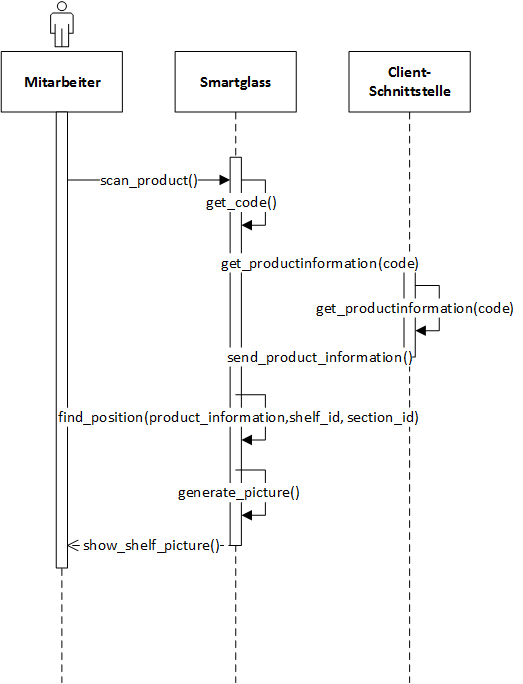
\includegraphics[scale=0.8]{Bilder/Abbildungen/SMAR_produkt_finden_Sequenzdiagramm.png}}
	\caption{Sequenzdiagramm Produkt finden}
	\label{fig:jwt_encode}
\end{figure}
Nachdem der Mitarbeiter die Funktion gestartet hat, vermittelt er der Smartglass den Befehl ein Produkt zu finden, sodass die Smartglass sofort in den Scan-Modus springt (scan\_product()). Dabei hat der Mitarbeiter die Intention, dass die Smartglass ihm dabei Hilft den Regalplatz zu finden.

Sofern der Artikel gescannt wurde, berechnet die Smartglass aus dem Bild den entsprechenden Code (get\_code()). Dies geschieht mit der ZingLibrary. Nachdem die Smartglass den Code errechnet hat, verschickt sie diesen Code an den Datenbankserver, der sich im gleichen Netzwerk befindet, damit dieser mit Produktinformationen antwortet. Mithilfe des Codes sucht die Datenbank intern zuerst nach dem entsprechenden Produkt. Anschließend werden über das Produkt folgende Informationen zurück an die Smartglass geschickt:
\begin{itemize}
	\item Der Name zur ergonomischen und leichten Handhabung für den Mitarbeiter.
	\item Die Füllstände von dem Artikel auf der Verkaufsfläche und im  Lager.
	\item Die aktuell ausgewählte Unit (Karton, Einzelstück).
	\item Das zugehörige Shelf als auch die entsprechende Section.
\end{itemize}
Der Name sowie die Füllstände im Lager und im Verkauf werden dem Nutzer angezeigt.

Mithilfe der Produktinformation, um welches Produkt es sich handelt, und der hinterlegten Karte aller Produktplätze generiert die Smartglass ein Bild – genauer eine SVG Grafik (generate\_picture()). Die Smartglass hat intern eine Karte mit den Attributen Shelf und Section. Dies sind Unterteilungen der Grafik in entsprechende Bereiche. Die Brille weiß allerdings nicht, welches Produkt in welchem Shelf, Section Paar liegt. Mithilfe der Datenbank erfährt sie diese Informationen und kann mit der lokal gespeicherten Karte, das Bild erzeugen. Dieses Bild zeigt einen Ausschnitt des Regalplatzes und markiert den Bereich, in dem das Produkt einzuräumen ist. Dieses Bild wird dem Mitarbeiter anschließend angezeigt. (send\_shelf\_picture()).

Da in den meisten Fällen nach der Produktplatz suche, das jeweilige Produkt eingeräumt werden soll, fragt die Brille den Mitarbeiter, ob er dies tun möchte.
Bestätigt er, springt sozusagen der Instruction Pointer in den Prozess „Produkt einräumen“. Dort wird allerdings der Scan-Vorgang übersprungen und öffnet den Dialog mit schon getroffenen Produktinformationen. 
Verneint der Nutzer, so springt die Smartglass zurück an den Anfang vom „Produkt finden“ Prozess. 

\subsection{Produkt einräumen}
Dieser Abschnitt gibt Implementierungsdetails sowie architektonische Einblicke in die Umsetzung des Prozesses „Produkt einräumen“. Dabei soll die Umsetzung chronologisch beschrieben werden mit zur Hilfenahme des folgenden Sequenzdiagramms. Vorausgesetzt ist, dass der Mitarbeiter schon die Funktion „Produkt einräumen“ ausgewählt hat. 
\begin{figure}[H]
	\centering
	{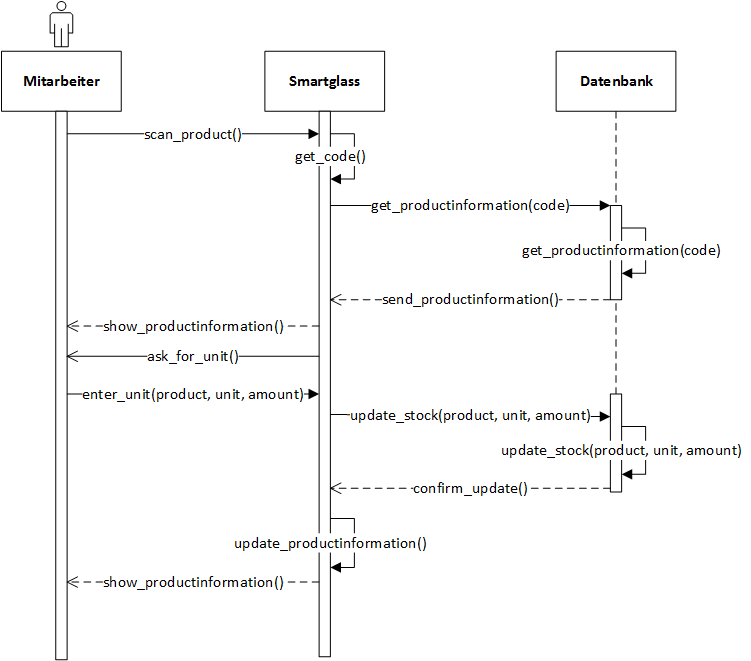
\includegraphics[scale=0.7]{Bilder/Abbildungen/SMAR_produkt_einraeumen_Sequenzdiagramm.png}}
	\caption{Sequenzdiagramm Produkt einräumen}
	\label{fig:jwt_encode}
\end{figure}
Ähnlich dem Prozess, Produkt finden, gibt es drei Aktoren, den Mitarbeiter, die Smartglass und die Datenbank, und startet, indem der Nutzer den \glqq Produkt einräumen\grqq -Prozess gestartet hat (scan\_product()). Daraufhin startet die Smartglass den Barcodescanner und berechnet aus dem erfassten Bild einen Code (get\_code()). Dieser Code wird an die Datenbank verschickt mit der Aufforderung produktspezifische Informationen anzugeben (get\_productinformation()). Die Datenbank sucht diese Informationen raus und antwortet der Smartglass mit diesen (send\_productinformation()). Bei diesen Informationen handelt es sich um folgende: 
\begin{enumerate}
	\item Der Name zur ergonomischen und leichten Handhabung für den Mitarbeiter.
	\item Die Füllstände von dem Artikel auf der Verkaufsfläche und im  Lager.
	\item Die aktuell gescannte Unit (Karton, Einzelstück).
\end{enumerate}
Die gescannte Unit ist dabei der Barcode an einem Karton oder einem einzelnen Produkt. So kann die einzuräumende Unit, und damit Menge, vorselektiert werden. 

Diese Informationen werden dem Mitarbeiter auf dem Display angezeigt. Dies ist auch der Punkt an dem der Prozess \glqq Produkt finden\grqq , in diesen Prozess springt.

So muss der Mitarbeiter weniger mit der Smartglass interagieren. Er hat allerdings noch die Möglichkeit die Unit entsprechend anzupassen (ask\_for\_unit() und enter\_unit()). Dabei hat der Mitarbeiter auch die Möglichkeit nicht nur die Unit anzugeben (ob Karton oder Einzelstück), sondern direkt die Möglichkeit eine Anzahl anzugeben (\zB 4 Kartons). Damit soll die mehrfache Interaktion vermieden werden. 

Schließlich bestätigt der Mitarbeiter (enter\_unit()) und die Smartglass leitet die neuen Informationen an die Datenbank weiter (update\_stock()). So werden dort die Füllstände für das Lager und auf der Verkaufsfläche entsprechend angepasst (update\_stock()).

Die Datenbank bestätigt dies (confirm\_update()), die Smartglass aktualisiert die Informationen, die dem Nutzer angezeigt werden (die Füllstände) (show\_productinformation()), und springt schließlich zurück zum Anfang des Prozesses. 



\subsection{Warenannahme}
Dieser Abschnitt beschreibt den Interaktionsprozess zwischen dem Mitarbeiter, der Smartglass und der Datenbank. Wie in den vorherigen Abschnitten wird ein Sequenzdiagramm zur Illustrierung verwendet. Voraussetzung für diesen Prozess ist, dass der Mitarbeiter den Prozess "Warenannahme" im Hauptmenü ausgewählt hat. 
\\
Ist dies geschehen öffnet die Smartglass den Scanmodus und erwartet vom Mitarbeiter, dass dieser den Lieferschein einscannt. Der Lieferschein ist deshalb wichtig, damit die folgenden Waren, die angenommen werden, der korrekten Lieferung zugeordnet werden können (scan\_delivery\_note()). 
\\
Wurde der Code eingescannt, wird intern der Code berechnet und ein Request an die Datenbank geschickt (get\_delivery\_information()). Dabei wird der gescannte Code mitgeschickt. Die Datenbank überprüft den Code und sucht die erwartenden Produkte und Mengen heraus (get\_delivery\_information()). Diese sendet die Datenbank als Response zurück an die Smartglass (send\_information()), welche diese dem Mitarbeiter anzeigt (show\_delivery\_information()).
\\
Wie in der Schleife zu sehen, wiederholt sich der folgende Vorgang solang bis entweder der Lieferschein abgearbeitet ist oder der Mitarbeiter diesen unterbricht. Bis dahin Scannt der Mitarbeiter jeden Artikel bzw. Karton (scan\_product()). Daraufhin berechnet die Smartglass den Code, verschickt diesen an die Datenbank, sodass diese den Lagerbestand entsprechend anpasst. Sofern die Datenbank aus dem Code das Produkt zugeordnet hat (get\_product()), wird der Wert entsprechend aktualisiert (update\_stock()). Anschließend werden Bestätigungen bis runter zum Mitarbeiter verschickt und angezeigt.
\\
Hat der Mitarbeiter den Lieferschein abgearbeitet, wird eine kurze Erfolgsmeldung angezeigt, damit der Mitarbeiter eine Rückmeldung bekommt (success\_delivery\_scan()).

\begin{figure}[H]
	\centering
	{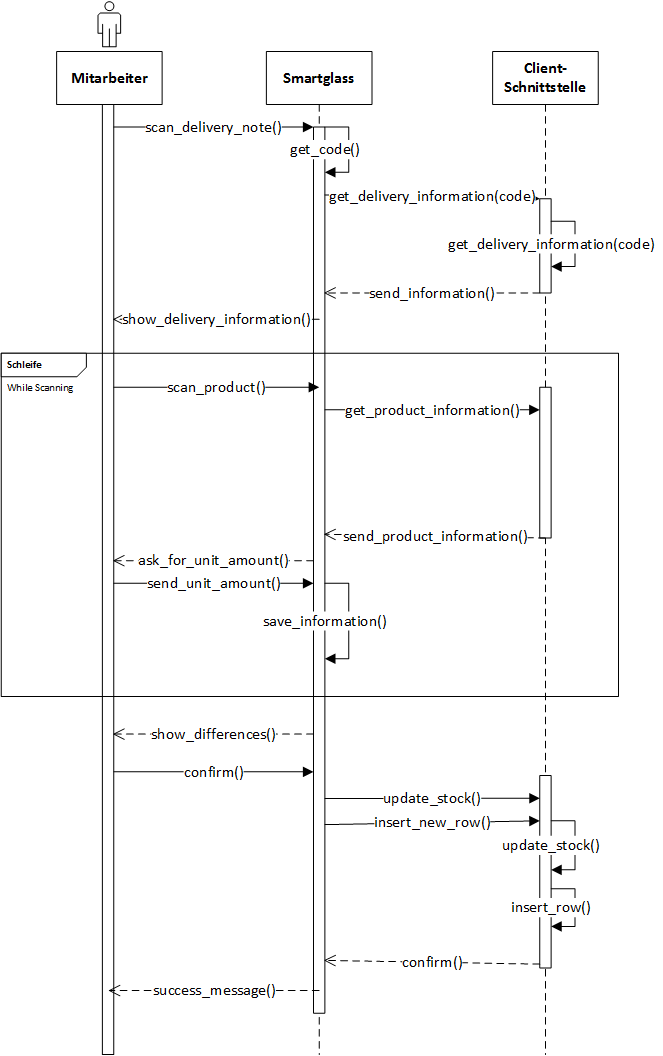
\includegraphics[scale=1.0]{Bilder/Abbildungen/SMAR_warenannahme_Sequenzdiagramm.png}}
	\caption{Sequenzdiagramm Produkt einräumen}
	\label{fig:sequenz_warenannnahme}
\end{figure}

\section{HTTP Nutzung}
\label{sec:httpnutzung}
Dieser Abschnitt befasst sich nicht mit einem konkreten Prozess, sondern erklärt das allgemeine vorgehen und die Akteure bei einem der vielen REST API Aufrufe. Voraussetzungen für eine einwandfrei Nutzung der REST API sind zwei Pakete auf der Smartglass notwendig. Diese sind standardmäßig ausgeliefert und müssen somit nicht manuell nachinstalliert werden.
\begin{enumerate}
	\item org.apache.http
	\item org.json.JSONObject
\end{enumerate}
Das erste Paket stellt die Hauptklassen und -methoden zur Nutzung von HTTP Komponenten. Diese sind essentiell, um das HTTP Protokoll zu verwenden. Es stellt zum Beispiel über HTTP die Verbindung auf und bietet die Möglichkeiten Requests zu versenden und Responses entgegen zu nehmen.\footnote{\citep{http}} Grundsätzlich ist zu sagen, dass hier nur eine schematische und vereinfachte Erklärung gewählt ist. 
\\
Das zweite Paket bietet Möglichkeiten JSON Objekte zu erstellen und mit diesen zu arbeiten. \footnote{\citep{json}}
\\
Das folgende Klassendiagramm visualisiert die nötigen Klassen, um einen HTTP Request zu schicken, eine Antwort zu erhalten und schließlich die Informationen davon, zu verwenden.
\begin{figure}[H]
	\centering
	{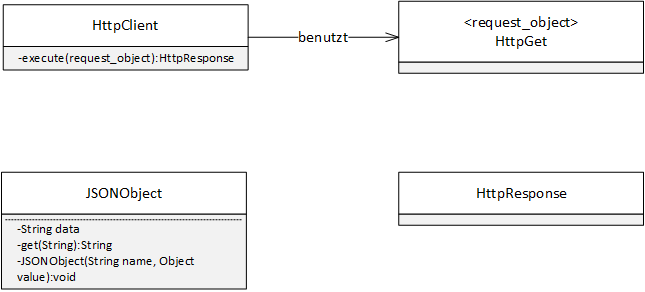
\includegraphics[scale=0.7]{Bilder/Abbildungen/http_request_klassendiagramm.png}}
	\caption{HTTP Request Klassendiagramm}
	\label{fig:sequenz_warenannnahme}
\end{figure}
Zu Beginn wird ein Objekt der Klasse \glqq HttpClient\grqq erzeugt. Der HttpClient kann ein sogenanntes \glqq request\_object\grqq verwenden. In der Grafik ist es konkret ein \glqq HttpGet\grqq -Objekt, das erzeugt wird. Grundsätzlich sind aber auch HttpPost, HttpDelete und HttpPut, nur um die wichtigsten HTTP Verben zu nennen, möglich. In einer Instanz der Klasse HttpGet wird eine URL zugewiesen, und anschließend benutzt das Objekt HttpClient, mithilfe der \glqq execute\grqq -Methode, das request\_object.
\\
Wird dieser Befehl ausgeführt, so wird ein Http-Request an den Server geschickt. Dieser antwortet mit einem einfach HttpResponse, bestehend aus Header und Body. Sofern der Request korrekt und ohne Fehler durchlaufen ist, ist der Body des Response nicht leer. Somit kann er mithilfe eines Objekts der Klasse HttpResponse angenommen werden. Prinzipiell ist darin ein String enthalten. 
\\
Wie in einem vorherigen Kapitel schon angesprochen, sind die HttpResponses in diesem konkreten Projekt in JSON Syntax geschrieben. Deshalb ist der String im \glqq HttpResponse\grqq Objekt in JSON Syntax, sodass sich dieser leicht verwerten sollte. Dies ist mithilfe eines JSON Objekts einfach. Dazu wird die Methode bzw. auch der Konstruktor mit dem entsprechendem String gefüllt. Die Umwandlung des String in einzelne Attribute übernimmt das Objekt selbst. Mithilfe der Methode \glqq get(String)\grqq können einzelne Attribute herausgezogen werden, indem als \glqq String\grqq der Name des Attributes angegeben wird.
\\
Somit lassen sich die vielen Http-Aufrufe, also die Interaktion mit den hinterlegten REST Services, sehr einfach und elegant nutzen und verarbeiten.

\section{Settings}
\label{sec:settings}
Dieser Abschnitt beschreibt und erklärt die Umsetzung des Speicherungsmechanismus auf der Smartglass. Hierzu wird die Klasse \glqq PreferencesHelper.java\grqq erläutert. 
\\
Prinzipiell werden in einer Applikation unter einer Android-Umgebung Informationen in einem sogenannten SharedPreferences-Pool gespeichert. Diese sind einer Aktivität zugeordnet, haben einen Namen und einen Wert. Dazu wird der Pool der aktuellen Aktivität geladen und über einen Editor editierbar gemacht. So können Einstellungen verändert werden. 
\\
Ähnlich ist das Abrufen von Einstellungen. Dazu wird ebenfalls über die aktuelle Aktivität der \glqq SharedPreferences\grqq aufgerufen, und darin der Name der Einstellung herausgesucht. Anschließend erhält man den Wert der Einstellung. 
\\
Es wurde sich dafür entschieden die oben erwähnte Klasse zu implementieren, um eine Abstraktionsschicht für jegliche Zugriffe auf Einstellungen zu gewährleisten. So laufen alle Zugriffe gleich ab, und bei Änderungen oder Erweiterungen gibt es einen zentralen Ort. Dennoch sind alle nutzenden Klassen von Veränderungen betroffen. 
\\
Konkret sind Standardmaßnahmen für den Lesenden sowie Schreibenden Zugriff auf Einstellung mit den Parameter String als auch Integer. Diese scharfe Trennung muss auch erfolgen, da der Editor nur genaue Typen akzeptiert. 



\section{Projektdefinition}
Kapitel \ref{cha:intro}

\section{Aufbau der Arbeit}
\subsection{bla}
\subsubsection{blabla}
\textbf{bla}\\
Hochkommata: \glqq asdas\grqq~~ sdasd\\

Neue Zeile: nur Backslash Backslash\\
sadas\\

Absatz\\

Aufzählung:
\begin{itemize}
	\item basd
	\item ...
\end{itemize}

\textit{\textbf{yxcyxcyxc}}
\underline{sdfsdf}
$\rightarrow$





